%! TEX root = ../000-main.tex
\chapter{Non-parametric regression model}
\chaptermark{NP reg. model}

\section{Introduction}

\begin{definition}{Regression function}{}

	Let $(X,\, Y)$ be random variables with continuous joint distribution.

	The best prediction (in the sense of the minimum mean squared prediction error)
	of the dependent variable $Y$ given that the independent variable $X$ takes
	the known value $x$ is the conditional expectation of $Y$ given $X=x$:
	\begin{equation*}
		m(x) = \mathds{E}( Y \mid X = x)
	\end{equation*}
	also known as \iemph{regression function}.
\end{definition}

\subsection{Parametric regression model}

The \iemph{parametric regression model} assumes that the regression function
is known except for a fixed finite number of parameters.

\begin{example}{Simple linear regression model}{}
	\begin{equation*}
		y = \beta_0 + \beta_1 X + \varepsilon
	\end{equation*}
	So the regression function is $m(x) = \beta_0 + \beta_1 x$ is known except
	for the parameters $\beta_0$ and $\beta_1$.
\end{example}

\subsection{Non-parametric regression model}

In the \iemph{non-parametric regression model} the functional form of the
regression function $m(x)$ is not specified.

\begin{note}
	However, certain regularity conditions are assumed. For instance,
	it is usually assumed that $m(x)$ has a continuous second derivative.
\end{note}

\begin{question}{What does it mean to fit a non-parametric regression model?}{}
	To provide an estimator $\hat{m}(t)$ of the regression function $m(t)$ for
	all $t \in \mathbb{R}$.

	This usually implies to draw the graphic of the pairs $(t,\, \hat{m}(t))$ where
	$t_j,\, j=1,\ldots,J$ is a regular fine grid covering the range of observed values
	$x_i,\, i=1,\ldots,n$.
	Alternatively, an algorithm that computes the values $\hat{m}(t)$ for any $t$
	can be provided.

	We also have give an estimator $\hat\sigma^2$ of the residual variance $\sigma^2$.
\end{question}

\pagebreak
\section{Local polynomial regression}
\subsection{Local linear regression}

\paragraph{Initial idea} Divide the range of $X$ into $K$ disjoint intervals
each of them showing an \iemph{approximately linear} relationship between $X$ and $Y$.
\begin{figure}[H]
	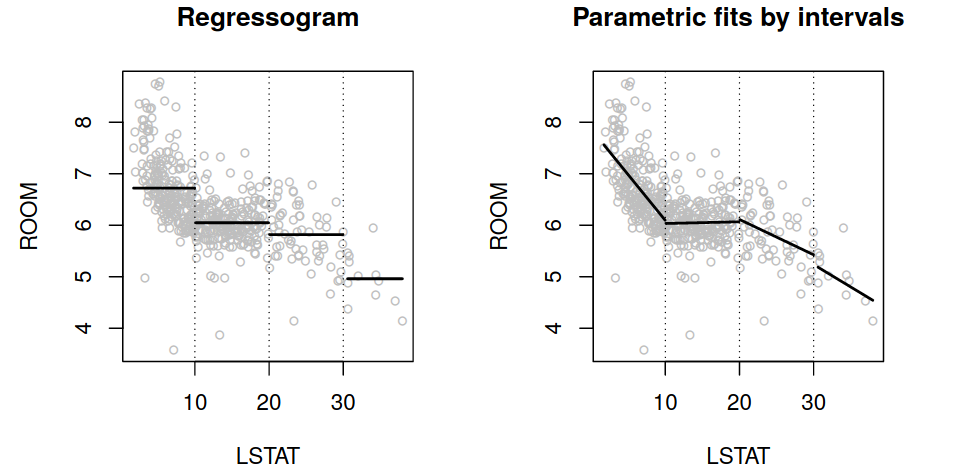
\includegraphics{ll_init}
	\caption{Initial idea of local linear regression.}
\end{figure}

This provides good results, but its not satisfactory, we apply to improvements:
\begin{description}
	\item[Localizing] In order to estimate the regression function at a given value $t$,
		use the data $(x_i,\, y_i)$ such that $x_i$ is in an interval centered at $t$.
	\item[Smoothing] Assign to each datum $(x_i,\, y_i)$ a weight $w_i$ that decreases
		as $|x_i - t|$ increases.
\end{description}

\begin{definition}{datum}{}
	A datum is a pair $(x_i,\, y_i)$ where $x_i$ is the value of the independent
	variable and $y_i$ is the value of the dependent variable.
\end{definition}

\subsubsection{Local linear fitting}
Weights are assigned by a \iemph{kernel function} $K$: usually a
symmetric unimodal density function centered at $0$.

The weight of $(x_i, y_i)$ is when estimating $m(t)$ is:
\begin{equation*}
	w_i = w(t,\,x_i) = K \left. \left( \frac{x_i - t}{h} \right) \middle/ \sum_{j=1}^n K \left( \frac{x_i - t}{h} \right) \right.
\end{equation*}
where $h$ is the \iemph{smoothing parameter} or \iemph{bandwidth}.

\begin{note}
	The final estimate is significantly affected by the choice of the bandwidth, so this
	choice is crucial in non-parametric estimation.
\end{note}

\begin{figure}[H]
	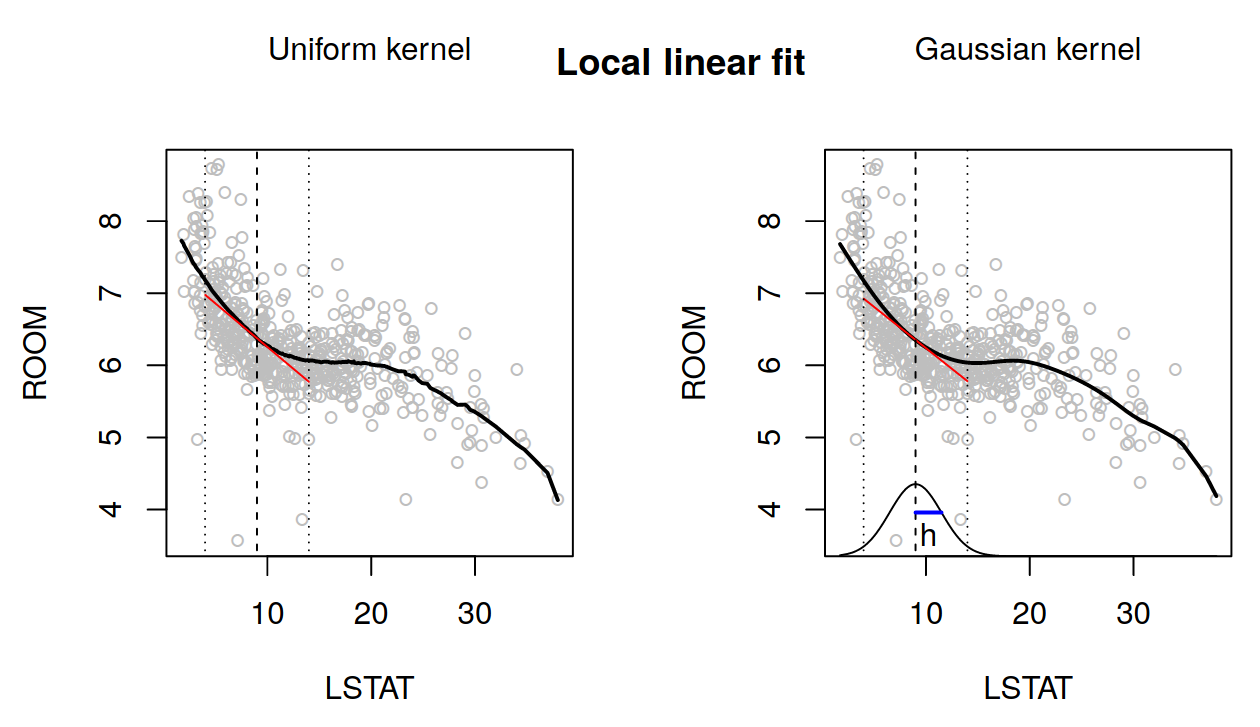
\includegraphics{ll_fit}
	\caption{Local linear fit with different kernel choices.}
\end{figure}

\subsection{Local polynomial regression}
Consider the weighted polynomial regression problem:
\begin{problem}{Weighted polynomial regression problem}{}
\begin{equation*}
	\min_{\beta_0,\ldots,\beta_q} \mathlarger{\sum_{i=1}^n} w_i \left( y_i - \beta_0 - \sum_{j=1}^q \beta_j x_i^j \right)^2
\end{equation*}
\end{problem}
Observe that the estimated coefficients depend on $t$, the
point for which the regression function is being estimated: $\hat\beta_j = \hat\beta_j(t)$.

The proposed estimate for $m(t)$ is the value of the locally fitted
polynomial $P_{q,t}(x) = \sum_{j=0}^q \hat\beta_j(x - t)^j$ at $x = t$:
\begin{equation*}
	\hat{m}(t) = P_{q,t}(t) = \hat\beta_0(t)
\end{equation*}

Moreover, the estimated polynomial $P_{q,t}(x)$ allows us to estimate the first $q$ derivatives
of $m$ at $t$:
\begin{equation*}
	\hat{m}_q^{(r)}(t) = \frac{d^r}{dx^r} P_{q,t}(t) {\Bigm|_{x=t}} = r! \hat\beta_r(t)
\end{equation*}

\subsubsection{Particular case: Nadaraya-Watson estimator}
\begin{definition}{Nadaraya-Watson estimator}{}
	When the degree of the locally fitted polynomial is \emph{$q=0$} (i.e. a constant),
	the resulting non-parametric estimator is called \iemph{Nadaraya-Watson estimator}
	or \iemph{kernel estimator}:
	\begin{equation*}
		\hat m_K(t) = \frac{
			\sum_{i=1}^n K \left( \frac{x_i - t}{h} \right) y_i
		}{
			\sum_{i=1}^n K \left( \frac{x_i - t}{h} \right)
		} = \sum_{i=1}^n w(t, x_i) y_i
	\end{equation*}
	\tcblower

	This was proposed before local polynomial estimators.

	\begin{note}
		\paragraph{Observe:} $\hat m_K(t)$ is a \iemph{moving weighted average}.
	\end{note}

\end{definition}


\begin{prop}{Every local polynomial estimator is itself a weighted average}{}
	\begin{equation*}
		\hat m_{q}(t) = \sum_{i=1}^n w_q^*(t,\, x_i) y_i
	\end{equation*}
	But the weights $w_q^*(t,\, x_i)$ are not necessarily non-negative.
\end{prop}

\subsubsection{Matrix formulation of the local polynomial estimator}
Let
\begin{equation*}
	X_t = \begin{pmatrix}
		1      & x_1 - t & \ldots & (x_1 - t)^q \\
		1      & x_2 - t & \ldots & (x_2 - t)^q \\
		\vdots & \vdots  & \ddots & \vdots      \\
		1      & x_n - t & \ldots & (x_n - t)^q
	\end{pmatrix}
\end{equation*}
be the \iemph{regressor matrix}.

We define $Y = (y_1, \ldots, y_n)^T,\, \varepsilon = (\varepsilon_1, \ldots, \varepsilon_n)^T,\,
	\beta = (\beta_0, \ldots, \beta_q)^T$ and we let $W_t = \text{diag}(w(x_1, t), \ldots, w(x_n,t))$
be the \iemph{weight matrix}.

We fit the regression model $Y = X_t\beta + \varepsilon$ using weighted least squares:
\begin{align*}
	\hat\beta & = \argmin_{\beta\in\mathbb{R}^{q+1}} \sum_{i=1}^n w_i(y_i - \beta_0 - \sum_{j=1}^q \beta_j x_i^j)^2 \\
	          & = \argmin_{\beta\in\mathbb{R}^{q+1}} (Y - X_t\beta)^T W_t (Y - X_t\beta)
\end{align*}
The solution is:
\begin{equation*}
	\hat\beta = (X_t^T W_t X_t)^{-1} X_t^T W_t Y
\end{equation*}

For $j=0,\ldots,q$, let $e_j$ be the $(q+1)$-dimensional vector
having all its coordinates 0 except for the $(j+1)$-th one, which is 1.
Then:
\begin{equation*}
	\hat m_q(t) = \hat \beta_0 = e_0^T (X_t^T W_t X_t)^{-1} X_t^T W_t Y = S_tY = \sum_{i=1}^n w^*_q(t,\, x_i) y_i
\end{equation*}
where $S_t = e_0^T (X_t^T W_t X_t)^{-1} X_t^T W_t$ is an $n$-dimensional row vector (it
is in fact a \iemph{smoothing matrix}).

\begin{note}
	We say that the local polynomial regression estimator is a \iemph{linear smoother}
	because for a fixed $t$, $\hat m_q(t)$ is a linear function of $y_1,\ldots,y_n$.
\end{note}

The local polynomial estimator of the $r$-th derivative of $m$ at point $t$ is:
\begin{equation*}
	\hat m_q^{(r)}(t) = r!e_r^T\hat\beta_r(t) = r!e_r^T\hat\beta
\end{equation*}
which is also linear in $y_1,\ldots,y_n$.

\subsection{Linear smoothers}

\begin{definition}{Linear smoother}{}
	A non-parametric linear regression estimator $\hat m$ is said to be
	a \iemph{linear smoother} when for any fixed $t$, $\hat m(t)$ is a linear function of
	$y_1,\ldots,y_n$:
	\begin{equation*}
		\hat m(t) = \sum_{i=1}^n w(t, x_i) y_i
	\end{equation*}
	for some weight function $w$.
	\tcblower
	\begin{note}
		Linear smoothers are particular cases of linear estimators of the regression
		function, as \iemph{OLS} or \iemph{ridge regression}.
	\end{note}
\end{definition}

\begin{definition}{Smoothing matrix}{}

	Let
	\begin{equation*}
		\hat y_i = \hat m (x_i) = \sum_{j=1}^n w(x_i, x_j) y_j
	\end{equation*}
	be the fitted values for the $n$ observed values  $x_i$ of the explanatory variable.

	In matrix format:
	\begin{equation*}
		\hat Y = S Y
	\end{equation*}
	where column vectors $Y$ and $\hat Y$ have elements $y_i$ and $\hat y_i$ respectively,
	and the matrix $S$ has generic element $s_{ij} = w(x_i, x_j)$.

	\begin{note}
		The matrix $S$ is called the \iemph{smoothing matrix}, because its effect on the observed
		data $(x_i, y_i)$ is to transform them into $(x_i, \hat y_i)$ which is a much
		smoother data configuration.
	\end{note}

	\tcblower
	The smoothing matrix is analogous to the \iemph{hat matrix} $H = X(X^TX)^{-1}X^T$ in
	multiple linear regression:
	\begin{equation*}
		\hat Y = X(X^TX)^{-1}X^T Y = H Y
	\end{equation*}
\end{definition}

\begin{prop}{Parameters in a linear smoother model}{effective-parameters}
	For a linear smoother with smoothing matrix $S$, the \iemph{effective
		number of parameters} is the sum of diagonal elements of $S$:
	\begin{equation*}
		\nu = \text{Trace}(S) = \sum_{i=1}^n s_{ii}
	\end{equation*}
	\tcblower
	\begin{note}
		The interpretation of $\nu$ as the effective number of parameters is
		valid for any linear non-parametric estimator.
	\end{note}

	We can thus compare the degree of smoothing of two linear non-parametric
	estimators just by comparing their effective number of parameters.
\end{prop}

\subsubsection{An estimator of $\sigma^2$}
An estimator of $\sigma^2$ in non-parametric estimation is:
\begin{equation*}
	\hat\sigma^2 = \frac{1}{n-\nu} \sum_{i=1}^n (y_i - \hat m(x_i))^2
\end{equation*}

\subsection{Kernel functions}

\begin{definition}{Kernel functions}{}
	Density functions with zero mean.
	\tcblower
	We can also rescale them so that they have zero mean and
	variance 1. Then we call them \iemph{rescaled kernels}.
\end{definition}

\begin{figure}[H]
	% 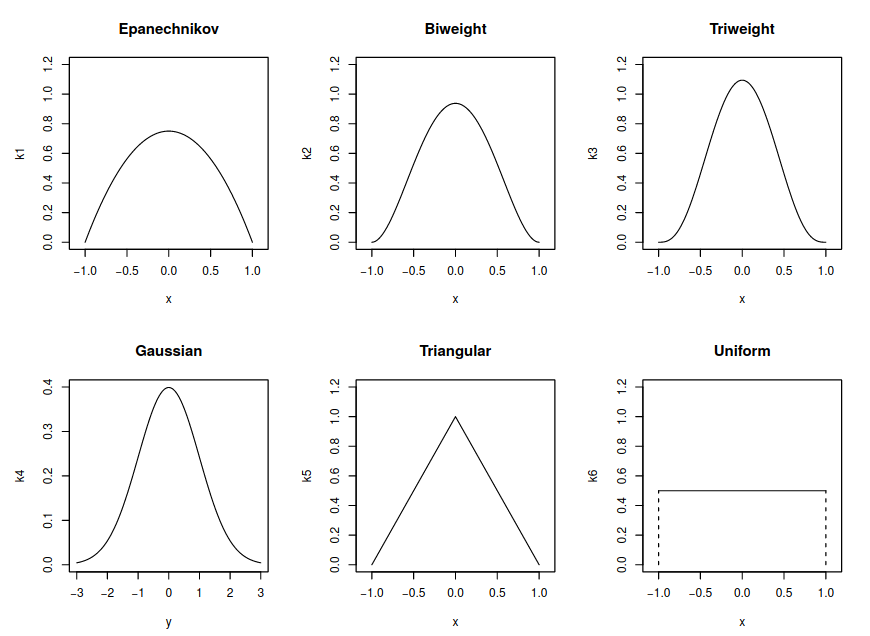
\includegraphics{kernel_examples}
	\begin{tikzpicture}
		\begin{groupplot}[group style={
						group size=3 by 2,
						xlabels at=edge bottom,
						ylabels at=edge left,
                        vertical sep=4em,
					},
				width = .3\textwidth,
				ymin=-0.1, ymax=1.1,
				xlabel=$x$, ylabel=$K(x)$,
                every axis plot/.append style={mark=none, line width=2pt},
                samples=50,
                domain=-1:1,
                xmin=-1.2, xmax=1.2
			]
            \nextgroupplot[title={\bfseries Epanechnikov ($K^*$)}]
			\addplot[ color=blue] {3/4*(1-x^2)*((x>=-1)*(x<=1))};

			\nextgroupplot[title={\bfseries Biweight}]
			\addplot[ color=red] {15/16*(1-x^2)^2*((x>=-1)*(x<=1))};

			\nextgroupplot[title={\bfseries Triweight}]
			\addplot[ color=green!70!black] {35/32*(1-x^2)^3*((x>=-1)*(x<=1))};

			\nextgroupplot[title={\bfseries Gaussian},xmin=-3.7, xmax=3.7]
			\addplot[domain=-3:3, color=orange] {1/sqrt(2*pi)*exp(-x^2/2)*2};

			\nextgroupplot[title={\bfseries Triangular}]
            \draw[line width=2pt, color=black] (-1,0) -- (0,1) -- (1,0);

			\nextgroupplot[title={\bfseries Uniform}]
            \draw[line width=2pt, color=gray] (-1,0.5) -- (1,0.5);
            \draw[line width=2pt, color=gray,dashed] (-1,0) -- (-1,0.5);
            \draw[line width=2pt, color=gray,dashed] (1,0) -- (1,0.5);
		\end{groupplot}
	\end{tikzpicture}
	\caption{Examples of Kernel functions used in non-parametric estimation}
\end{figure}

\begin{table}[H]
	\caption{Examples of Kernel functions used in non-parametric estimation}
	\begin{tabular}{lccl}
		\toprule
		Kernel ($K$)         & Expression                                & Variance & Efficiency \\
		\midrule
		Epanechnikov ($K^*$) & $\frac{3}{4}(1-x^2)I_{[-1,1]}(x)$         & $1/5$    & 1          \\
		Biweight             & $\frac{15}{16}(1-x^2)^2I_{[-1,1]}(x)$     & $1/7$    & 0.994      \\
		Triweight            & $\frac{35}{32}(1-x^2)^3I_{[-1,1]}(x)$     & $1/9$    & 0.987      \\
		Gaussian             & $\frac{1}{\sqrt{2\pi}}e^{-\frac{x^2}{2}}$ & $1$      & 0.951      \\
		Triangular           & $\frac{1}{2}(1-|x|)I_{[-1,1]}(x)$         & $1/6$    & 0.986      \\
		Uniform              & $\frac{1}{2}I_{[-1,1]}(x)$                & $1/3$    & 0.930      \\
		\bottomrule
	\end{tabular}
\end{table}

\subsection{Theoretical properties of local polynomial regression}

\subsubsection{Local Properties}

The \iemph{local behaviour} refers to the statistical properties of
a non-parametric estimate $\hat m(t)$ as estimator of the unknown
value $m(t)$ at a given point $t$.

\begin{definition}{Bias}{Bias}
	Let $m(t)$ be the true value of the regression function at $t$.
	The \iemph{bias} of a non-parametric estimator $\hat m(t)$ is:
	\begin{equation*}
		\text{Bias}_{m(t)}(\hat m(t)) = \mathbb E[\hat m(t)] - m(t)
	\end{equation*}
\end{definition}

\begin{definition}{Variance}{Variance}
	The \iemph{variance} of a non-parametric estimator $\hat m(t)$ is:
	\begin{equation*}
		\text{Var}_{m(t)}(\hat m(t)) = \mathbb E\bigl[(\hat m(t) - \mathbb E[\hat m(t)])^2\bigr]
	\end{equation*}
\end{definition}

\begin{definition}{Mean Squared Error (MSE)}{MSE}
	The \iemph{mean squared error} of a non-parametric estimator $\hat m(t)$ is:
	\begin{equation*}
		\text{MSE}_{m(t)}(\hat m(t)) = \mathbb E\bigl[(\hat m(t) - m(t))^2\bigr]
		= \text{Bias}_{m(t)}(\hat m(t))^2 + \text{Var}_{m(t)}(\hat m(t))
	\end{equation*}
\end{definition}

\begin{question}{Local properties}{}
	\begin{itemize}
		\item Is $\hat m (t)$ an unbiased estimator of $m(t)$? ($\text{Bias}_{m(t)}(\hat m(t)) = 0$)
		\item Is $\lim_{n\to\infty}\text{Var}_{m(t)}(\hat m(t)) = 0$?
		\item Is $\hat m (t)$ a consistent estimator of $m(t)$? Does $\hat m (t)$ converge to $m(t)$?
		\item Is $\lim_{n\to\infty}\text{MSE}_{m(t)}(\hat m(t)) = 0$?
	\end{itemize}
\end{question}

\subsubsection{Global Properties}

We talk about \iemph{global properties} when our interest is on $\hat m(t)$
as an estimator of $m(t)$ for all $t \in [a, b]$, where $[a, b]$ is the
interval where the explanatory variable $x$ takes its values.

\begin{question}{Global properties}{}
	Does the estimated function $\hat m$ converge to the unknown function $m$
	in some sense appropriate for functions?
	\tcblower
	One common way for measuring the distance between $\hat m$ and $m$ is
	the \emph{Integrated Mean Squared Error} (IMSE):
	\begin{equation*}
		\lim_{n\to\infty} \text{IMSE}_{m}(\hat m) = 0?
	\end{equation*}
\end{question}

\begin{definition}{Integrated Mean Squared Error (IMSE)}{IMSE}
	\begin{align*}
		\text{IMSE}_{m}(\hat m) & = \int_a^b \text{MSE}_{m(t)}(\hat m(t)) \, dt
		= \int_a^b \mathds{E}\bigl[(\hat m(t) - m(t))^2\bigr] \, dt                  \\
		                        & = \int_a^b \text{Bias}_{m(t)}(\hat m(t))^2 \, dt +
		\int_a^b \text{Var}_{m(t)}(\hat m(t)) \, dt
	\end{align*}
\end{definition}

\begin{theorem}{Bias and Variance of $\hat m_0(t)$ and $\hat m_1(t)$}{}
	Consider the non-parametric regression model:
	\begin{equation*}
		Y_i = m(X_i) + \varepsilon_i, \quad i = 1, \ldots, n
	\end{equation*}
	where $\varepsilon_1, \ldots, \varepsilon_n$ are independent r.v. with
	$\text{Var}(\varepsilon_i) = \sigma^2(x_i)$; $X_1, \ldots, X_n$ are
	independent r.v. with density $f$ and $P(a \leq X_i \leq b) = 1$ for some
	$a, b \in \mathbb R$. Assume the following regularity conditions:
	\begin{enumerate}
		\item $f(t) > 0\quad\forall t$.
		\item $f(t),\, m''(t)$ and $\sigma^2(t)$ are continuous in the neighborhood of $t$.
		\item $K$ is symmetric with support on $[-1, 1]$, $\int_R K(u) \, du = 1$ and
		      $\int_{-1}^1 K(u) \, du = 0$.
		\item $t \in (a, b)$.
		\item $h \to 0$ and $n\cdot h \to \infty$ when $n \to \infty$.
	\end{enumerate}
	\tcbline
	In this context, the following statements hold:
	\begin{enumerate}
		\item The \iemph{Nadaraya-Watson estimator} and the \iemph{local linear estimator}
		      both have the variance:
		      \begin{equation*}
			      \frac{\sigma^2(t)}{nhf(t)} \int_{-1}^1 K^2(u) \, du + o\left(\frac{1}{nh}\right)
		      \end{equation*}
		\item The \emph{Nadaraya-Watson estimator} has bias:
		      \begin{equation*}
			      \left(
			      \frac{m'(t)f'(t)}{f(t)} + \frac{m''(t)}{2}
			      \right)h^2
			      \int_{-1}^1 u^2K(u) \, du + o\left(h^2\right)
		      \end{equation*}
		\item The \emph{local linear estimator} has bias:
		      \begin{equation*}
			      \frac{m''(t)}{2} h^2
			      \int_{-1}^1 u^2K(u) \, du + o\left(h^2\right)
		      \end{equation*}
		\item The $\text{MSE}_{m(t)}(\hat m(t))$ is $O(h^4) + O(1/(nh))$ for both estimators.
		      Then, both converge to $m(t)$ in quadratic mean and in probability.
	\end{enumerate}
\end{theorem}

\subsubsection{Bias-Variance Tradeoff}
\begin{definition}{Asymptotic Mean Squared Error (AMSE)}{AMSE}\index{AMSE}\index{asymptotic mean squared error}
	Is the main part of the MSE (ignoring the infinitesimal terms).
\end{definition}

Let us consider the AMSE for the local linear estimator:
\begin{equation*}
	\text{AMSE}(h) = \underbrace{\frac{(m''(t))^2}{4}h^4 \left( \int_{-1}^1 u^2 K(u)\, du \right)^2}_{\text{bias}^2}
	+
	\underbrace{\frac{\sigma^2(t)}{nhf(t)} \int_{-1}^1 K^2(u) \, du}_{\text{variance}}
\end{equation*}

The first term, the squared bias, increases with $h$.

The second term, the variance, decreases with $h$.

\begin{note}
	The optimal value $h_{\text{AMSE}}$ represents the compromise between bias and variance.
\end{note}

\begin{figure}[H]
	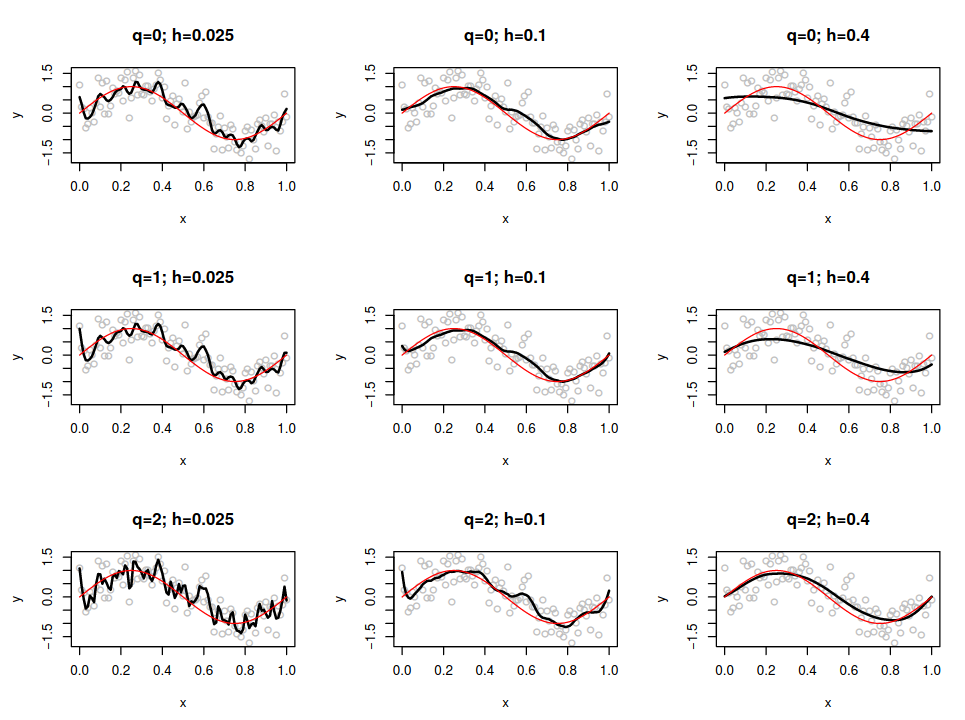
\includegraphics{effect_hq}
	\caption{Effect of bandwidth $h$ and degree $q$ on a single sample.}
\end{figure}

\subsection{Choosing the Smoothing Parameter (Bandwidth)}
The choice of the smoothing parameter $h$ is a crucial step in the appearance
and properties of the regression function estimator.

\begin{description}
	\item[Estimation]
		The bandwidth controls the \iemph{Bias-Variance Tradeoff}. With a small bandwidth,
		the estimator is highly variable and has small bias. With a large bandwidth, the
		opposite happens.
	\item[Prediction of New Observations] The smoothing parameter $h$ controls the
		balance between fitting the observed data well and the ability to predict
		new observations.

		Small values of $h$ give more flexibility, but the prediction errors
		will be higher (\iemph{overfitting}).

		If $h$ is too large, there is \iemph{underfitting}, as it may happen with
		global parametric models. In this case, both the errors in the observed data
		and the prediction will be high.
\end{description}

\paragraph{Criteria for Choosing the Smoothing Parameter}
There are several sensible criteria for choosing the smoothing parameter. We can
categorize them in two groups:
\begin{enumerate}
	\item \emph{Estimation quality} based methods (statistical perspective).
	\item \emph{Prediction error} based methods (machine learning perspective).
\end{enumerate}

\subsubsection{Estimation based criteria}

\paragraph{Integrated Mean Squared Error (IMSE)} We can minimize the
IMSE (\ref{def:IMSE}) to choose the bandwidth $h$ as shown in~\cref{fig:IMSE}.
\begin{figure}[H]
	\includegraphics{IMSE}
	\caption{IMSE for different values of $h$.}%
	\label{fig:IMSE}
\end{figure}

\begin{definition}{Mean Integrated Squared Error (MISE)}{MISE}\index{MISE}\index{mean integrated squared error}
	\begin{equation*}
		\text{MISE}(\hat m) = \mathds{E}_{\boldsymbol Z} \left[
			\int_a^b \left( m(t) - \hat m(t) \right)^2 f(t) \, dt
			\right] =
		\mathds{E}_{\boldsymbol Z} \left[
			\mathds{E}_T \left\{
			\left( m(T) - \hat m(T) \right)^2 \mid \boldsymbol Z
			\right\}
			\right]
	\end{equation*}
	where $\boldsymbol Z = \left\{(x_i,\, Y_i) \mid i = 1,\ldots,n\right\}$ is the sample
	used to estimate $\hat m$ and $T$ is a r.v. independent from $\boldsymbol Z$
	with the same distribution that generates the independent variable values $x_i$.
	\tcblower
	\begin{note}
		It coincides with IMSE by \iemph{Fubini's Theorem}.
	\end{note}
\end{definition}

\subsubsection{Prediction based criteria}
\begin{definition}{Predictive Mean Squared Error (PMSE)}{PMSE}\index{PMSE}\index{predictive mean squared error}
	Is the expected squared error made when predicting $Y = m(t) + \varepsilon$ by $\hat m(t)$.
	Where $t$ is an observation of the r.v. $T$, distributed as the observed explanatory variable.

	When $T$ and $\varepsilon$ are independent from the sample $\boldsymbol Z$, then:
	\begin{align*}
		\text{PMSE}(\hat m) & = \mathds{E}_{\boldsymbol Z,(T,Y)} \left[
			\left(Y - \hat m(T)\right)^2
			\right]
		= \mathds{E}_{\boldsymbol Z,T,\varepsilon} \left[
			\left(\hat m(T) - m(T) - \varepsilon\right)^2
		\right]                                                         \\
		                    & = \mathds{E}_{\boldsymbol Z,T} \left[
			\left(\hat m(T) - m(T)\right)^2
			\right] + \mathds{E}_\varepsilon\left[\varepsilon^2\right]
		= \text{MISE}(\hat m) + \sigma^2
	\end{align*}
	\tcblower
	\begin{note}
		MISE and PMSE are equivalent when $T$ and $\varepsilon$ are independent from $\boldsymbol Z$.
	\end{note}
\end{definition}

\begin{marker}
	Unfortunately, both IMSE, MISE and PMSE are \emph{unfeasible} to compute
	because they require the knowledge of the \emph{true} regression function
	$m$ (which is unknown in practice).
\end{marker}

\begin{definition}{Residual Sum of Squares (RSS)}{RSS}\index{RSS}\index{residual sum of squares}
	Is an \emph{optimistic} estimation of PMSE:
	\begin{equation*}
		\text{RSS}(\hat m) = \frac{1}{n} \sum_{i=1}^n \left( Y_i - \hat m(x_i) \right)^2
	\end{equation*}
	\tcblower
	\begin{note}
		Also known as the \iemph{error in the training sample}
	\end{note}
\end{definition}

Only the RSS is feasible to compute, but it is not a good estimator of PMSE
since it is \emph{optimistically} biased.

\subsubsection{Bandwidth Selection in Practice}
As we have seen, the proposed criteria are not feasible to compute. We have several
alternatives based in a train, test (and validation) split of the data.
\begin{itemize}
	\item Minimizing the average squared prediction error in a validation set.
	\item Leave-one-out cross-validation.
	\item K-fold cross-validation.
	\item Generalized cross-validation (Only for linear estimators)
\end{itemize}

\begin{definition}{Validation set}{}
	When the available data is large enough, we can randomly split it into
	3 sets:
	\begin{enumerate}
		\item \iemph{Training set}: Used to fit the model.
		\item \iemph{Validation set}: Used for model selection and parameter tuning.
		\item \iemph{Test set}: Used to evaluate the generalization of the final model.
	\end{enumerate}
\end{definition}

\begin{definition}{$\text{PMSE}_\text{Val}$}{PMSEVal}
	We can choose the bandwidth $h_\text{Val}$ by minimizing the
	Predictive Mean Squared Error in the validation set:
	\begin{equation*}
		\text{PMSE}_\text{Val}(h) = \frac{1}{n_V} \sum_{i=1}^{n_V} \left( Y_i^V - \hat m(x_i^V) \right)^2
	\end{equation*}
	where $(x_i^V,\, Y_i^V),\,i=1,\ldots,n_V$ are the observations of the validation set and
	$\hat m$ is the estimator with bandwidth $h$ using the training set.
\end{definition}

\begin{definition}{Leave-one-out cross-validation (LOOCV)}{LOOCV}
	\begin{enumerate}
		\item For each observation $(x_i,\, Y_i)$ of the training set, we fit the model
		      using the remaining observations.
		\item We compute the squared prediction error for the observation $(x_i,\, Y_i)$
		      using the fitted model.
		\item We average the squared prediction errors.
	\end{enumerate}
	\begin{equation*}
		\text{PMSE}_\text{LOOCV}(h) = \frac{1}{n} \sum_{i=1}^n \left( Y_i - \hat m_h(x_i) \right)^2
	\end{equation*}
	\tcblower
	\begin{note}
		LOOCV is a good alternative when the number of observations is small and we cannot
		afford to split the data into 3 sets.
	\end{note}
	\begin{note}
		LOOCV is a special case of K-fold cross-validation with $K=n$.
	\end{note}
	\begin{note}
		$\text{PMSE}_\text{LOOCV}(h)$ is an approximately unbiased estimator of $\text{PMSE}(h)$,
		but has a high variance.
	\end{note}
\end{definition}

\begin{definition}{$K$-fold cross-validation}{}
	Instead of taking one observation, we split the training set into $K$ subsets
	and remove whole subsets at each iteration.

	\tcblower
	\begin{note}
		$K$-fold cross-validation has lower variance than LOOCV, but larger bias.
	\end{note}
	Usually we use $K=5$ or $K=10$.
\end{definition}

\begin{definition}{Generalized cross-validation (GCV)}{GCV}
	For linear smoothers, a modification can be done in the measure
	of $\text{PMSE}_\text{CV}$.

	It consists in replacing the values of $s_{ii}$ coming
	from the diagonal of $S$ in the definition of
	$\text{PMSE}_\text{CV}$ by their average value $\nu/n$:
	\begin{equation*}
		\text{PMSE}_\text{GCV}(h) = \frac{1}{n} \sum_{i=1}^n \left(
		\frac{y_i - \hat y_i}{1 - \nu/n}
		\right)^2
	\end{equation*}
	Where $\nu = \text{Trace}(S) = \sum_{i=1}^n s_{ii}$ is the number of effective
	parameters (prop.~\ref{prop:effective-parameters}).

	We can further simplify the expression to:
	\begin{equation*}
		\boxed{
			\text{PMSE}_\text{GCV}(h) = \frac{n\hat\sigma_\varepsilon^2}{n - \nu}
		}
	\end{equation*}
	where $\hat\sigma_\varepsilon^2 = \frac{1}{n-\nu}\sum^n_{i=1}\left(y_i - \hat y_i\right)^2$
	estimates the residual variance.
\end{definition}

\subsection{Choosing the degree of the local polynomial}
The effect on the final estimation of the degree of the
local polynomial is \emph{much less} important
than the choice of the bandwidth. We can follow the following
recommendations:
\begin{itemize}
	\item The larger the $q$, the better asymptotic properties in bias,
	      but in general its recommended to use $q = r+1$ where $r$ is the
	      order of the derivative of $m$ that is estimated.
	\item It is preferable to use \emph{odd} degree.
	\item To decide between cubic or linear, we take into account the
	      expression of the local linear estimator bias. Bias is high
	      in intervals where the function has high curvature ($m''$).
	      If we suspect that the regression function $m$ could be very
	      bumpy, it would be better to use $q=3$.
\end{itemize}
